

\chapter{Stability study}
\label{ch:Stability study}

define the stability of the rotational motion of the obejct???

System definition and model: The system is composed of an undeformable rotating object and a modular robot made out of identical spherical modules. The robots moves and deploys itself at the surface of the object by maintianing contact at all time. As the rotational motion is the only focus of this study, the system is considered to be isolated\gls{ghc}.
The best way to model is to use 

Write..\gls{ghc}.


\section{System modelling}
\label{System modelling}

Write.. \gls{pe}.

Write.. \glspl{pe}.

\section{Hamiltonian Lagrange formulation}
\label{Hamiltonian Lagrange formulation}

Write.. \gls{pe}.

Write.. \glspl{pe}.

\begin{figure}[h]
 \begin{center}
 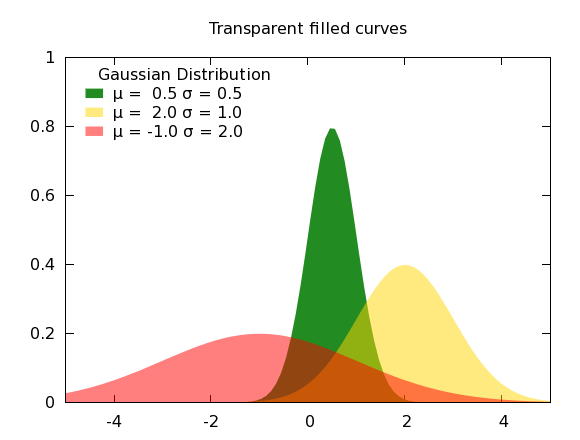
\includegraphics [width=12cm]{Figures/Background/pic.png}
 \caption{Figure Caption.}
 \label{fig:label}
\end{center}
\end{figure} 

\cite{gum, ghc-smp}

\subsection{Subsection}

\begin{table}[h]
\begin{center}
\begin{tabular}{c c c c} % centered columns (4 columns)
\hline\hline %inserts double horizontal lines
Case & Method\#1 & Method\#2 & Method\#3 \\ [0.5ex] % inserts table 
%heading
\hline % inserts single horizontal line
1 & 50 & 837 & 970 \\ % inserting body of the table
2 & 47 & 877 & 230 \\
3 & 31 & 25 & 415 \\
4 & 35 & 144 & 2356 \\
5 & 45 & 300 & 556 \\ [1ex] % [1ex] adds vertical space
\hline %inserts single line
\end{tabular}\caption{Table Caption}
\label{tab:lable}
\end{center}
\end{table}


\subsubsection{Subsubsection}